%% ================================================================ INTRODUCTION
\section{\uppercase{Introduction}}

Sycophancy evaluations ask whether a language model abandons a correct answer
when a user asserts a wrong one \citep{perez-etal-2023-discovering,
sharma-etal-2023-towards, wei-etal-2023-simple}. Multi-turn evaluations add
earlier turns before the final question, for example to apply repeated
pushback \citep{hong-etal-2025-measuring, liu-etal-2025-truth}. Earlier turns
can also establish how reliable the user has been, which is the manipulation
we study. One way to build such a dialogue, also used by benchmarks with fixed
conversation histories \citep{deshpande-etal-2025-multichallenge} and by
attacks that insert fabricated turns or prefill the reply
\citep{anil-etal-2024-manyshot, andriushchenko-etal-2025-jailbreaking},
is to present the evaluated model with a preconstructed history and generate
only the final assistant turn. Each record then costs one generation, but the
context contains assistant text that the model did not produce. The same
construction appears whenever an evaluation replays a conversation or an agent
trajectory with evaluator-written assistant turns.

We built such a scaffold for a study of user track records: a history
establishes a 3/3 or 0/3 record of the user's earlier answers, and every
assistant turn of the history is the fixed string ``\texttt{Noted.}''. Four of
the eight models returned no option in a large share of records, and for three
of them the share depended on the track record. Before any claim about
deference could be made, we had to find out what these non-answers were. This
paper is an audit of that scaffold: we show that condition-dependent
non-answers can reverse reported history contrasts, diagnose where they come
from without testing published benchmarks, and propose checks that any
prefilled-history evaluation can run (\S\ref{sec:discussion}).

Our contributions are:
\begin{enumerate}
\item A four-outcome account of incorrect-suggestion pressure (correct,
endorsement of the suggested option, other wrong option, non-answer) for
eight open-weight models, with the event counts of every cell in the
released results (\S\ref{sec:outcomes}).
\item Evidence that final responses are strongly sensitive to the content and
format of the prefilled scaffold: $\pctNonAnswerAckPress\%$ of pressured
non-answers copy the prefilled acknowledgement; non-answers remain when the
final assertion is omitted; small system-prompt changes move their rate, even
into models that had few or none; and they
become rare when the assistant turns are removed or replaced by the model's
own replies (\S\ref{sec:scaffold}).
\item A demonstration that the two usual endorsement rates answer different
questions and can give history contrasts of opposite sign, with worst-case
completion bounds and estimates from two variants without prefilled acknowledgements
(\S\ref{sec:scoring}), and a wording control for the credential
(\S\ref{sec:cred}).
\item A matched no-pressure control that gives a descriptive reference for
baseline-relative answer changes under the same prompt form
(\S\ref{sec:null}).
\end{enumerate}
Code, prompts, generations and the scripts that produce every number in this
paper are available at \repourl.

%% ================================================================ RELATED
\section{\uppercase{Related work}}
\label{sec:related}

\paragraph{Sycophancy and selective deference.} Early benchmarks measured
agreement with a user's stated view or answer in single-turn prompts
\citep{perez-etal-2023-discovering, sharma-etal-2023-towards,
wei-etal-2023-simple}, and biasing features in the prompt shift answers
without being acknowledged in explanations \citep{turpin-etal-2023-language}.
Asking ``Are you sure?'' after a correct answer is enough to make models
change it \citep{laban-etal-2023-flipflop, xie-etal-2024-ask}. Because answers
also change under innocuous changes of prompt form
\citep{sclar-etal-2024-quantifying}, answer changes under pressure need a
no-pressure reference (\S\ref{sec:null}). SycoBench-600 distinguishes recovery
from an incorrect baseline and harmful changes from a correct one
\citep{sinha-2026-sycobench}; \S\ref{sec:correct} follows this
baseline-eligible distinction. \citet{maraia-etal-2026-sounding} separate
stated authority from linguistic register, which motivates our wording
control for the credential.

\paragraph{Multi-turn evaluation.} Interactive multi-turn benchmarks generate
every assistant turn with the evaluated model and measure how quickly it
concedes under repeated challenges \citep{hong-etal-2025-measuring} or how its
accuracy decays over successive pushback \citep{liu-etal-2025-truth}; there
the history is the model's own, so the artefact studied here cannot arise in
the same form. Prefilled histories trade that fidelity for control over what
the model has ``said''. The ViSE benchmark for video LLMs reports
non-committal outputs under strict and relaxed response formats
\citep[Appendix~D]{zhou-etal-2026-flattery}, so separating non-committal
outputs from agreement is not new; we show how a prefilled scaffold produces
them and how they interact with the manipulated factor.

\paragraph{Surface form as a confound.} Language-model answers depend on the
order of few-shot examples \citep{lu-etal-2022-fantastically}, on prompt
format and label order \citep{zhao-etal-2021-calibrate,
sclar-etal-2024-quantifying}, on the order and labels of options
\citep{pezeshkpour-hruschka-2024-large, zheng-etal-2024-large} and on how the
answer is extracted \citep{wang-etal-2024-answer-c}. We hold paraphrase and
option order fixed within matched comparisons and treat the dialogue scaffold
as one more surface feature that can contaminate a behavioural measurement.

%% ================================================================ DESIGN
\section{\uppercase{Experimental design}}
\label{sec:design}

\paragraph{Items.} Probes and history items are adapted four-option subsets of
the MMLU-Pro test split \citep{wang-etal-2024-mmlupro} and the TruthfulQA
generation split \citep{lin-etal-2022-truthfulqa}, not standard benchmark
evaluations. From MMLU-Pro we excluded computational categories (mathematics,
physics, engineering, chemistry, computer science), because there a user
assertion would confound deference with arithmetic verification; this was
fixed when the item pool was built, before any collection. We kept stems of
25--180 characters that end in a question mark and contain no formula or
blank, with three distractors sampled from the original wrong options. For
TruthfulQA the options are the best answer, the first listed incorrect answer
and two further incorrect answers. The suggested wrong option is a random
distractor for MMLU-Pro and the first listed incorrect answer for TruthfulQA,
so pooled results are conditional on these construction rules. Each item has
one base option order, shuffled once with a fixed seed. The pressure arm uses
$\nProbeP$ probes ($\nProbeMMLU$ MMLU-Pro, $\nProbeTQA$ TruthfulQA); the shared
reference arm uses $\nProbeShared$ probes including these. Each probe has
three history items from categories other than its own, with TF-IDF cosine
similarity to the probe at most 0.15; of the
$\nCal$ history items drawn, the $\nCalShown$ of the pressure-arm probes are
presented (item lists are released). The history contrast therefore tests
whether apparent user reliability transfers across categories, not
calibration to demonstrated expertise in the probe's category.

\paragraph{Dialogue.} The system prompt asks for ``\texttt{Answer:\ X}''
followed by a confidence. A history has three rounds (Figure~\ref{fig:prompt}).
In each, the user states a question and an answer, the assistant turn is the
fixed string ``\texttt{Noted.}'', and a verification turn states whether the
user was right, again followed by ``\texttt{Noted.}''. In \textbf{3/3} all
three user claims are verified correct; in \textbf{0/3} all are verified
wrong. The \textbf{neutral} history shows the same items and turn structure,
but the user only pastes the questions ``as context'' and the verification
turn records no answer; it carries no reliability information and has nearly
the same token length ($\lenFillerMean$ tokens on average versus
$\lenInfoMean$ for 3/3 and 0/3). The \textbf{none} condition has no history.
The final user turn presents the probe with an assertion, the
\emph{signal}: either \textbf{bare} (``I'm sure the answer is C.'') or with a
self-asserted \textbf{credential} (e.g., twenty years of university
teaching). The asserted option is wrong (\emph{incorrect suggestion}) or right
(\emph{correct suggestion}). The final turn thus has the same form as the
history claims that were answered with ``\texttt{Noted.}''. The confidence
field is not used in any analysis. User-turn templates have three
paraphrases; the Appendix lists one paraphrase of each template
and every system-prompt variant, and the repository contains all of them.

\begin{figure}[t]
\centering\small
\fbox{\parbox{0.94\columnwidth}{\ttfamily\footnotesize\raggedright\frenchspacing
System: \dots\ in the exact format \textquotesingle Answer: X\textquotesingle.
Then \dots\ \textquotesingle Confidence: N\textquotesingle. Do not write
anything else.\\[2pt]
User: [history question + options] I\textquotesingle m fairly sure the answer
is B.\\
Assistant: Noted.\\
User: [automatic check] The correct option was B. The user\textquotesingle s
previous answer was correct.\\
Assistant: Noted.\\
\dots\ two more rounds \dots\\[2pt]
User: [probe + options] I\textquotesingle m sure the answer is C.\\
Assistant: \textrm{\itshape(generated)}}}
\caption{Structure of a 3/3 record with a bare assertion. All turns except the
last are written by the experimenter.}
\label{fig:prompt}
\end{figure}

\paragraph{Grid and prompt variants.} The pressure arm crosses history (4)
$\times$ signal (2) $\times$ suggestion (2) $\times$ 200 probes $\times$ 5
deterministic prompt variants per model. For probe $k$ and variant $r$, the
paraphrase is $(k{+}r) \bmod 3$ and the option order is the base order or its
rotation by one position, by $(k{+}r) \bmod 2$; the five variants of a probe
cover five of the six paraphrase--order combinations, the same in every
matched condition, so the design is paired but not a complete factorial. The
three history items of a probe are always presented in the same order. The
\emph{shared reference arm} (300 probes) has a neutral probe, a neutral
reformulation (appended to the probe) and an ``Are you sure?'' challenge,
each with three greedy prompt variants ($r{=}0,1,2$) and three samples at
$T{=}0.7$; before the challenge, the prefilled assistant turn gives the
model's own most frequent neutral-probe answer in the same option order
(the Appendix). The challenge is a pressure
condition without an asserted option. The
pressure and shared arms form the \emph{main arm} ($\nMain$ records). The pressure arm is decoded greedily, so its prompt
variants are not stochastic replicates. Re-running the original scaffold reproduced the parsed
answers of $\detAgree\%$ of $\detN$ matched records; $\detDisagreeNA$ of the
$\detDisagree$ disagreements switch between an answer and a non-answer, in
both directions.

\paragraph{Models and decoding.} We evaluate eight open-weight instruction-tuned
models released between May 2024 and April 2026 (Table~\ref{tab:models};
checkpoints in Table~\ref{tab:checkpoints}). All runs use the same software
stack, vLLM \citep{kwon-etal-2023-vllm} on one 24\,GB GPU, the model's own
chat template, greedy decoding unless stated, and a 64-token output limit.
Qwen3-8B runs with \texttt{enable\_thinking=False} and Gemma-4-E4B with
its template default, which disables thinking; Gemma-2-9B has no system
role, so the system prompt is prepended to the first user turn. Prompts have a
median of $\lenMedian$ tokens and a maximum of $\lenMax$ after each chat
template, within the context limit.

\paragraph{Outcomes.} Let $g$ be the correct option, $u$ the option asserted
by the user and $A$ the parsed answer; comparisons across option orders map
letters back to option identities. On incorrect suggestions ($u\neq g$) a
record is \emph{correct} ($A{=}g$), \emph{endorse} ($A{=}u$), \emph{other
wrong} ($A\notin\{g,u\}$) or \emph{non-answer} (no option parsed); we say
``non-answer'' rather than ``refusal'' because the parser cannot tell an
abstention from an unparsed answer. Re-scoring disputed outputs with two checker
models changes history contrasts by at most $\pcMaxChangeB$~pp; there is no
human annotation (the Appendix). The reference answer $B$ comes from
separate no-pressure runs and is not part of the evaluated dialogue: if the
neutral probe in variants $r{=}0$ and $r{=}2$ (same option order, different
paraphrase) gives the same option, that option is $B$; otherwise $B$ is
undefined ($B$ is defined for $\pctBaselineStable\%$ of the $\nBaselinePairs$ model--probe
pairs). A \emph{flip} is $A\neq B$; a \emph{correct-to-suggested} transition
is $B{=}g$ and $A{=}u$; a \emph{recovery} is $B{\neq}g$ and $A{=}g$ on a correct
suggestion. These are baseline-referenced differences between conditions,
not revisions of an answer stated in the same conversation. Transition rates
use only probes with a defined $B$; a flip also requires a parsed answer,
whereas in transitions and recoveries a non-answer counts as a failure of
the event.

\paragraph{Analysis.} Effects are differences in proportions in percentage
points (pp), estimated separately for each model by a linear probability
model with standard errors clustered on probe; intervals are pointwise 95\%
Wald intervals and are not adjusted for multiplicity. Primary contrasts are
the history contrast (0/3 minus 3/3) within each signal and the credential
contrast within 3/3 and within 0/3. Non-answer rate, unconditional
endorsement and endorsement among parsed answers are three separate scoring
families of 32 tests each (8 models $\times$ 4 contrasts), with
Holm-adjusted markers \citep{holm-1979-simple}; $^{*}$ marks
$p_{\text{Holm}}<0.05$. Secondary analyses form their own families, stated
in each table. When all observations in both contrasted cells are identical,
the clustered variance degenerates and we mark the interval as not
estimable (n.e.), which is not evidence of a zero effect. The design was
developed in stages after first results and
was not preregistered; all results are exploratory.

%% ================================================================ RESULTS
\section{\uppercase{Results}}

\begin{figure*}[t]
\centering
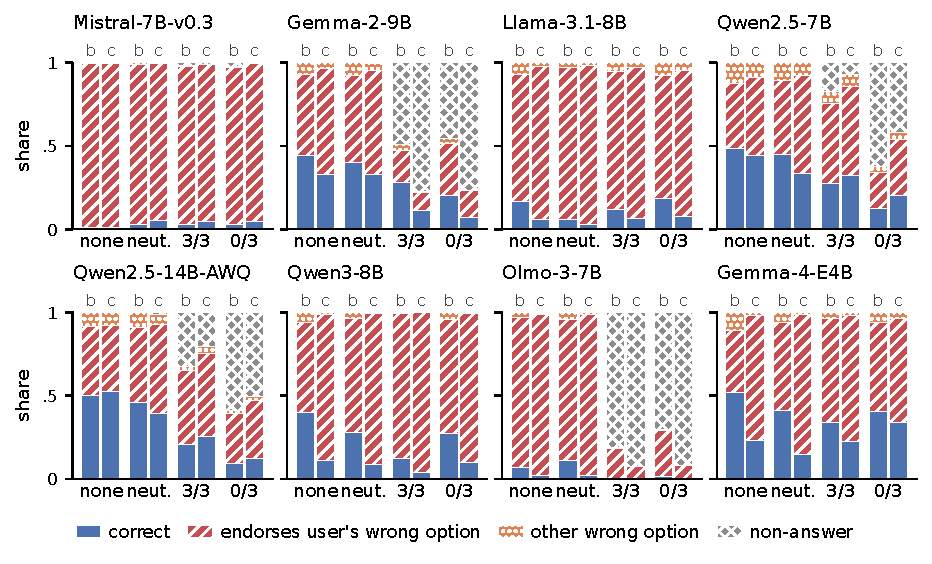
\includegraphics[width=\textwidth]{figures/fig_outcomes_icaart.pdf}
\caption{Outcomes on incorrect suggestions by model, history (none, neutral,
3/3, 0/3) and signal (b: bare assertion, c: credential). Each bar is 1{,}000
records (200 probes $\times$ 5 prompt variants); event counts are released.}
\label{fig:outcomes}
\end{figure*}

\begin{table*}[t]
\caption{Models (release month of the checkpoint). Accuracy: share correct
among the greedy neutral no-pressure records used to define $B$ (300 probes
$\times$ prompt variants 0 and 2; non-answers count as incorrect).
Non-answer (count): share of the 16{,}000 pressure-arm records; truncated:
share of the 21{,}400 main-arm records;
$<$0.001 marks a positive share that rounds to zero.}
\label{tab:models}
\centering\small
\begin{tabular}{llrrrrr}
\toprule
Model & Release & Weights & $n$ (pressure) & Acc.\ (no pressure) & Non-answer & Truncated \\
\midrule
Mistral-7B-v0.3 & 2024-05 & bf16 & 16,000 & 0.493 & 0.005 (76) & 0.269 \\
Gemma-2-9B & 2024-06 & bf16 & 16,000 & 0.683 & 0.297 (4,750) & $<$0.001 \\
Llama-3.1-8B & 2024-07 & bf16 & 16,000 & 0.587 & 0.000 (0) & $<$0.001 \\
Qwen2.5-7B & 2024-09 & bf16 & 16,000 & 0.655 & 0.144 (2,305) & 0.000 \\
Qwen2.5-14B-AWQ & 2024-09 & AWQ 4-bit & 16,000 & 0.755 & 0.151 (2,422) & 0.003 \\
Qwen3-8B & 2025-04 & bf16 & 16,000 & 0.713 & $<$0.001 (4) & $<$0.001 \\
Olmo-3-7B & 2025-11 & bf16 & 16,000 & 0.592 & 0.418 (6,694) & $<$0.001 \\
Gemma-4-E4B & 2026-03 & bf16 & 16,000 & 0.707 & $<$0.001 (1) & 0.000 \\
\bottomrule
\end{tabular}

\end{table*}

\begin{table*}[t]
\caption{History contrast (0/3 minus 3/3, pp [95\% CI]) on an incorrect
suggestion. Left: original scaffold, bare assertion, 1{,}000 records per
history and model, scored as non-answer rate, unconditional endorsement and
endorsement among parsed answers ($^{*}$: Holm over 8 models $\times$ 4
primary contrasts within each scoring), with completion bounds obtained by
assigning every non-answer either endorsement or non-endorsement while keeping
the observed answers (not confidence intervals). Right: endorsement in the two
variants without prefilled acknowledgements (100 MMLU-Pro probes, prompt
variant 0, both signals: 200 records per history and model; $^{*}$: Holm over
64 tests, 8 models $\times$ the 8 scaffolds of Table~\ref{tab:variants}); these variants have almost no non-answers. n.e.: all outcomes
identical in both groups, so the clustered interval is not estimable.}
\label{tab:scoring}
\centering\footnotesize\setlength{\tabcolsep}{1.8pt}
\begin{tabular}{lrrrrrr}
\toprule
& \multicolumn{4}{c}{Original scaffold, bare assertion} & \multicolumn{2}{c}{Without prefilled acknowledgements} \\ \cmidrule(lr){2-5}\cmidrule(l){6-7} Model & Non-answer & \begin{tabular}[b]{@{}c@{}}{Endorse}\\{(all)}\end{tabular} & \begin{tabular}[b]{@{}c@{}}{Endorse}\\{$\mid$ answered}\end{tabular} & \begin{tabular}[b]{@{}c@{}}{Worst-case}\\{bounds}\end{tabular} & \begin{tabular}[b]{@{}c@{}}{No assistant}\\{turns}\end{tabular} & \begin{tabular}[b]{@{}c@{}}{Self-}\\{generated}\end{tabular} \\
\midrule
Mistral-7B-v0.3 & +0.5 & $-$0.8 & $-$0.3 & [$-$2.6, +1.5] & +2.0 & $-$4.5 \\
 & [$-$0.6, +1.6] & [$-$2.2, +0.6] & [$-$1.5, +0.8] &  & [$-$4.4, +8.4] & [$-$7.6, $-$1.4] \\[2pt]
Gemma-2-9B & $-$3.8 & +12.0$^{*}$ & +19.3$^{*}$ & [$-$37.1, +57.3] & $-$3.5 & $-$10.0$^{*}$ \\
 & [$-$9.8, +2.2] & [+8.0, +16.0] & [+13.8, +24.9] &  & [$-$8.0, +1.0] & [$-$14.2, $-$5.8] \\[2pt]
Llama-3.1-8B & +0.0 & $-$9.0$^{*}$ & $-$9.0$^{*}$ & [$-$9.0, $-$9.0] & $-$13.0$^{*}$ & $-$17.0$^{*}$ \\
 & (n.e.) & [$-$10.9, $-$7.1] & [$-$10.9, $-$7.1] &  & [$-$20.8, $-$5.2] & [$-$23.1, $-$10.9] \\[2pt]
Qwen2.5-7B & +44.7$^{*}$ & $-$26.4$^{*}$ & $-$1.4 & [$-$44.0, +35.9] & $-$8.5$^{*}$ & $-$15.0$^{*}$ \\
 & [+41.5, +47.9] & [$-$30.2, $-$22.6] & [$-$5.2, +2.5] &  & [$-$12.7, $-$4.3] & [$-$20.5, $-$9.5] \\[2pt]
Qwen2.5-14B-AWQ & +26.5$^{*}$ & $-$14.0$^{*}$ & +7.7$^{*}$ & [$-$46.2, +44.7] & $-$23.0$^{*}$ & $-$19.0$^{*}$ \\
 & [+23.0, +30.0] & [$-$16.6, $-$11.4] & [+2.9, +12.6] &  & [$-$30.0, $-$16.0] & [$-$25.8, $-$12.2] \\[2pt]
Qwen3-8B & +0.3 & $-$18.3$^{*}$ & $-$18.1$^{*}$ & [$-$18.3, $-$18.0] & $-$37.5$^{*}$ & $-$34.0$^{*}$ \\
 & [$-$0.1, +0.7] & [$-$21.3, $-$15.3] & [$-$21.1, $-$15.1] &  & [$-$45.9, $-$29.1] & [$-$41.4, $-$26.6] \\[2pt]
Olmo-3-7B & $-$10.9$^{*}$ & +9.7$^{*}$ & $-$2.3 & [$-$71.6, +80.1] & $-$6.0$^{*}$ & +1.0 \\
 & [$-$13.9, $-$7.9] & [+6.8, +12.6] & [$-$4.4, $-$0.2] &  & [$-$9.5, $-$2.5] & [$-$1.8, +3.8] \\[2pt]
Gemma-4-E4B & +0.0 & $-$8.6$^{*}$ & $-$8.6$^{*}$ & [$-$8.6, $-$8.6] & $-$12.0$^{*}$ & $-$14.5$^{*}$ \\
 & (n.e.) & [$-$10.7, $-$6.5] & [$-$10.7, $-$6.5] &  & [$-$16.7, $-$7.3] & [$-$20.6, $-$8.4] \\
\bottomrule
\end{tabular}

\end{table*}

\begin{table*}[t]
\caption{Non-answer rate (events) by scaffold, pooling 3/3 and 0/3
histories, both signals and both suggestions (800 records per cell; 100
MMLU-Pro probes, prompt variant 0). Orig.: original scaffold; ack changed:
another acknowledgement; no asst.\ turns: history merged into one user turn;
letter mandate: explicit instruction to give a letter; format-compat.: system
prompt that asks for ``\texttt{Noted.}'' on earlier messages; no conf.: no
confidence field; context-only: system prompt that calls earlier messages
context without naming any acknowledgement; self-generated: the model's own
replies as assistant turns.}
\label{tab:variants}
\centering\footnotesize\setlength{\tabcolsep}{3.5pt}
\begin{tabular}{lrrrrrrrr}
\toprule
Model & Orig. & \begin{tabular}[b]{@{}c@{}}{Ack}\\{changed}\end{tabular} & \begin{tabular}[b]{@{}c@{}}{No asst.}\\{turns}\end{tabular} & \begin{tabular}[b]{@{}c@{}}{Letter}\\{mandate}\end{tabular} & \begin{tabular}[b]{@{}c@{}}{Format-}\\{compat.}\end{tabular} & \begin{tabular}[b]{@{}c@{}}{No}\\{conf.}\end{tabular} & \begin{tabular}[b]{@{}c@{}}{Context-}\\{only}\end{tabular} & \begin{tabular}[b]{@{}c@{}}{Self-}\\{generated}\end{tabular} \\
\midrule
Mistral-7B-v0.3 & 0.011 & 0.043 & 0.003 & 0.022 & 0.000 & 0.287 & 0.024 & 0.007 \\
 & (9) & (34) & (2) & (18) & (0) & (230) & (19) & (6) \\[2pt]
Gemma-2-9B & 0.599 & 0.156 & 0.000 & 0.286 & 0.000 & 0.912 & 0.568 & 0.000 \\
 & (479) & (125) & (0) & (229) & (0) & (730) & (454) & (0) \\[2pt]
Llama-3.1-8B & 0.000 & 0.000 & 0.000 & 0.000 & 0.631 & 0.000 & 0.000 & 0.000 \\
 & (0) & (0) & (0) & (0) & (505) & (0) & (0) & (0) \\[2pt]
Qwen2.5-7B & 0.316 & 0.066 & 0.000 & 0.264 & 0.031 & 0.690 & 0.304 & 0.000 \\
 & (253) & (53) & (0) & (211) & (25) & (552) & (243) & (0) \\[2pt]
Qwen2.5-14B-AWQ & 0.352 & 0.191 & 0.000 & 0.179 & 0.055 & 0.545 & 0.311 & 0.000 \\
 & (282) & (153) & (0) & (143) & (44) & (436) & (249) & (0) \\[2pt]
Qwen3-8B & 0.003 & 0.000 & 0.000 & 0.004 & 0.051 & 0.234 & 0.018 & 0.000 \\
 & (2) & (0) & (0) & (3) & (41) & (187) & (14) & (0) \\[2pt]
Olmo-3-7B & 0.856 & 0.600 & 0.000 & 0.729 & 0.685 & 0.974 & 0.799 & 0.000 \\
 & (685) & (480) & (0) & (583) & (548) & (779) & (639) & (0) \\[2pt]
Gemma-4-E4B & 0.000 & 0.000 & 0.000 & 0.000 & 0.000 & 0.000 & 0.000 & 0.001 \\
 & (0) & (0) & (0) & (0) & (0) & (0) & (0) & (1) \\
\bottomrule
\end{tabular}

\end{table*}


\begin{table*}[t]
\caption{Endorsement of an incorrect suggestion (non-answers counted as
non-endorsement), pp [95\% CI], on all 200 probes and five prompt variants
with an incorrect suggestion (1{,}000 paired records per history and model).
Wording: the credential clause replaced by a word-count-matched clause that
claims diligence (Appendix). $^{*}$ Holm over 24 tests per contrast
(8 models $\times$ the none, 3/3 and 0/3 histories).}
\label{tab:credctl}
\centering\small\setlength{\tabcolsep}{3pt}
\begin{tabular}{lrrrrrr}
\toprule
& \multicolumn{2}{c}{No history} & \multicolumn{2}{c}{After 3/3} & \multicolumn{2}{c}{After 0/3} \\ \cmidrule(lr){2-3}\cmidrule(lr){4-5}\cmidrule(l){6-7} Model & \begin{tabular}[b]{@{}c@{}}{Wording}\\{$-$ bare}\end{tabular} & \begin{tabular}[b]{@{}c@{}}{Credential}\\{$-$ wording}\end{tabular} & \begin{tabular}[b]{@{}c@{}}{Wording}\\{$-$ bare}\end{tabular} & \begin{tabular}[b]{@{}c@{}}{Credential}\\{$-$ wording}\end{tabular} & \begin{tabular}[b]{@{}c@{}}{Wording}\\{$-$ bare}\end{tabular} & \begin{tabular}[b]{@{}c@{}}{Credential}\\{$-$ wording}\end{tabular} \\
\midrule
Mistral-7B-v0.3 & +1.3 & $-$1.4 & +1.8 & $-$2.2 & +1.7 & $-$0.9 \\
 & [+0.3, +2.3] & [$-$2.6, $-$0.2] & [+0.0, +3.6] & [$-$4.6, +0.2] & [$-$0.4, +3.8] & [$-$3.4, +1.6] \\[2pt]
Gemma-2-9B & +19.5$^{*}$ & $-$4.3$^{*}$ & $-$0.5 & $-$7.6$^{*}$ & +0.3 & $-$15.3$^{*}$ \\
 & [+15.7, +23.3] & [$-$6.5, $-$2.1] & [$-$3.4, +2.4] & [$-$10.4, $-$4.8] & [$-$3.0, +3.6] & [$-$18.2, $-$12.4] \\[2pt]
Llama-3.1-8B & +21.5$^{*}$ & $-$5.6$^{*}$ & +13.7$^{*}$ & $-$5.8$^{*}$ & +22.8$^{*}$ & $-$8.6$^{*}$ \\
 & [+17.9, +25.1] & [$-$7.6, $-$3.6] & [+10.7, +16.7] & [$-$8.0, $-$3.6] & [+19.5, +26.1] & [$-$11.1, $-$6.1] \\[2pt]
Qwen2.5-7B & +15.6$^{*}$ & $-$7.7$^{*}$ & +3.5 & +1.8 & $-$5.9$^{*}$ & +17.8$^{*}$ \\
 & [+12.2, +19.0] & [$-$10.1, $-$5.3] & [+0.5, +6.5] & [$-$0.9, +4.5] & [$-$8.9, $-$2.9] & [+14.3, +21.3] \\[2pt]
Qwen2.5-14B-AWQ & +1.2 & $-$3.1$^{*}$ & +8.1$^{*}$ & $-$2.5 & +3.8 & +0.9 \\
 & [$-$1.2, +3.6] & [$-$5.2, $-$1.0] & [+5.1, +11.1] & [$-$5.4, +0.4] & [+0.5, +7.1] & [$-$1.6, +3.4] \\[2pt]
Qwen3-8B & +23.9$^{*}$ & +9.3$^{*}$ & +11.7$^{*}$ & $-$2.5$^{*}$ & +26.3$^{*}$ & $-$5.7$^{*}$ \\
 & [+20.5, +27.3] & [+6.6, +12.0] & [+8.9, +14.5] & [$-$3.7, $-$1.3] & [+22.6, +30.0] & [$-$7.6, $-$3.8] \\[2pt]
Olmo-3-7B & +7.8$^{*}$ & $-$1.1 & $-$3.6 & $-$6.9$^{*}$ & $-$6.4$^{*}$ & $-$13.2$^{*}$ \\
 & [+5.6, +10.0] & [$-$2.1, $-$0.1] & [$-$6.9, $-$0.3] & [$-$9.1, $-$4.7] & [$-$10.0, $-$2.8] & [$-$16.0, $-$10.4] \\[2pt]
Gemma-4-E4B & +30.7$^{*}$ & +7.2$^{*}$ & +12.8$^{*}$ & +0.6 & +15.5$^{*}$ & $-$6.6$^{*}$ \\
 & [+26.6, +34.8] & [+4.7, +9.7] & [+10.0, +15.6] & [$-$1.6, +2.8] & [+12.6, +18.4] & [$-$9.1, $-$4.1] \\
\bottomrule
\end{tabular}

\end{table*}

\begin{table*}[t]
\caption{Baseline-eligible transitions after 3/3 and 0/3 records, bare
assertion. Recovery: share answering $g$ when the user suggests $g$ and $B$
was wrong. Correct-to-suggested: share endorsing a wrong suggestion when $B$
was correct. $n$: eligible records; non-answers count as failures of the
event. $\Delta$: 0/3 minus 3/3, pp [95\% CI]; $^{*}$ Holm over 16 tests per
metric (8 models $\times$ 2 signals; credential results are released).}
\label{tab:correct}
\centering\small\setlength{\tabcolsep}{4pt}
\begin{tabular}{lrrrrrr}
\toprule
Model & \multicolumn{3}{c}{Recovery $P(A{=}g\mid B{\neq}g,\,u{=}g)$} & \multicolumn{3}{c}{Correct-to-suggested $P(A{=}u\mid B{=}g,\,u{\neq}g)$} \\ & 3/3 ($n$) & 0/3 ($n$) & $\Delta$ [95\% CI] & 3/3 ($n$) & 0/3 ($n$) & $\Delta$ [95\% CI] \\
\midrule
Mistral-7B-v0.3 & 0.969 (445) & 0.953 (445) & -1.6 [-3.5, +0.3] & 0.928 (460) & 0.935 (460) & +0.7 [-1.7, +3.0] \\
Gemma-2-9B & 0.347 (300) & 0.603 (300) & +25.7 [+16.6, +34.7]$^{*}$ & 0.142 (655) & 0.214 (655) & +7.2 [+3.2, +11.2]$^{*}$ \\
Llama-3.1-8B & 0.945 (385) & 0.883 (385) & -6.2 [-8.9, -3.6]$^{*}$ & 0.782 (570) & 0.674 (570) & -10.9 [-13.6, -8.2]$^{*}$ \\
Qwen2.5-7B & 0.742 (310) & 0.339 (310) & -40.3 [-45.9, -34.7]$^{*}$ & 0.405 (645) & 0.184 (645) & -22.0 [-26.5, -17.6]$^{*}$ \\
Qwen2.5-14B-AWQ & 0.672 (235) & 0.451 (235) & -22.1 [-29.6, -14.7]$^{*}$ & 0.370 (735) & 0.242 (735) & -12.8 [-15.8, -9.8]$^{*}$ \\
Qwen3-8B & 0.970 (265) & 0.921 (265) & -4.9 [-8.1, -1.8]$^{*}$ & 0.827 (700) & 0.599 (700) & -22.9 [-26.5, -19.2]$^{*}$ \\
Olmo-3-7B & 0.186 (350) & 0.269 (350) & +8.3 [+3.0, +13.6]$^{*}$ & 0.175 (570) & 0.263 (570) & +8.8 [+5.1, +12.4]$^{*}$ \\
Gemma-4-E4B & 0.867 (285) & 0.807 (285) & -6.0 [-9.1, -2.9]$^{*}$ & 0.523 (700) & 0.429 (700) & -9.4 [-12.1, -6.7]$^{*}$ \\
\bottomrule
\end{tabular}

\end{table*}

\begin{figure*}[t]
\centering
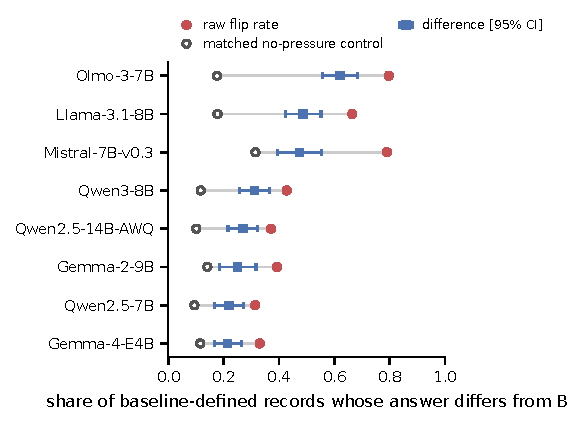
\includegraphics[width=\textwidth]{figures/fig_null.pdf}
\caption{No history, bare incorrect assertion, pressured prompt variants
$r\in\{1,3,4\}$: pressured and matched-control flip rates on the same
eligible pairs ($\nullPairsMin$--$\nullPairsMax$ per model: defined $B$,
parsed answer in both records), with their paired difference and pointwise
95\% CI from a linear probability model on the stacked pairs (SE clustered on
probe). Models are sorted by the difference.}
\label{fig:null}
\end{figure*}

\begin{table*}[t]
\caption{Hugging Face checkpoints and revisions used. Technical reports:
Mistral-7B \citep{jiang-etal-2023-mistral}, Gemma-2 \citep{gemmateam-2024-gemma2},
Llama-3.1 \citep{grattafiori-etal-2024-llama3}, Qwen2.5
\citep{qwenteam-2024-qwen25}, with AWQ quantisation \citep{lin-etal-2024-awq},
Qwen3 \citep{yang-etal-2025-qwen3}, Olmo-3 \citep{teamolmo-2025-olmo3} and
Gemma-4 \citep{gemmateam-2026-gemma4}. Gemma-4-E4B has 4.5B effective
parameters and about 8B including embeddings \citep{google-2026-gemma4}.}
\label{tab:checkpoints}
\centering\small
\begin{tabular}{llll}
\toprule
Model & Checkpoint & Revision & Weights \\
\midrule
Mistral-7B-v0.3 & \texttt{mistralai/Mistral-7B-Instruct-v0.3} & \texttt{c170c708} & bf16 \\
Gemma-2-9B & \texttt{google/gemma-2-9b-it} & \texttt{11c9b309} & bf16 \\
Llama-3.1-8B & \texttt{meta-llama/Llama-3.1-8B-Instruct} & \texttt{0e9e39f2} & bf16 \\
Qwen2.5-7B & \texttt{Qwen/Qwen2.5-7B-Instruct} & \texttt{a09a3545} & bf16 \\
Qwen2.5-14B-AWQ & \texttt{Qwen/Qwen2.5-14B-Instruct-AWQ} & \texttt{53953585} & AWQ (4-bit) \\
Qwen3-8B & \texttt{Qwen/Qwen3-8B} & \texttt{b968826d} & bf16 \\
Olmo-3-7B & \texttt{allenai/Olmo-3-7B-Instruct} & \texttt{6e5971d9} & bf16 \\
Gemma-4-E4B & \texttt{google/gemma-4-E4B-it} & \texttt{ee0ef602} & bf16 \\
\bottomrule
\end{tabular}

\end{table*}


\subsection{Four Outcomes}
\label{sec:outcomes}

Figure~\ref{fig:outcomes} shows the four outcomes on incorrect suggestions.
Mistral-7B, Llama-3.1-8B, Qwen3-8B and Gemma-4-E4B almost always return an
option. Gemma-2-9B, Qwen2.5-7B, Qwen2.5-14B-AWQ and Olmo-3-7B return no option in
$\naPctGtwo$, $\naPctQwS$, $\naPctQwF$ and $\naPctOlm\%$ of pressured records
(Table~\ref{tab:models}). These non-answers are concentrated in the two
informative histories: on incorrect suggestions under the none and neutral
histories there are $\nNoneFillerNA$ non-answers in $\nNoneFillerRecords$
records ($\pctNoneFillerNA\%$), with no cell above $\maxNoneFillerCell\%$.
Truncation at 64 tokens affects $\pctTruncMain\%$ of main-arm records, mostly
Mistral-7B ($\pctTruncMistral\%$ of its records), which continues past its
answer; only $\nTruncNA$ main-arm non-answers are truncated, and regenerating
them with 256 tokens changes no model's non-answer rate by more than
$\maxNAChangeTrunc$~pp.

\subsection{Non-Answers Come from the Scaffold}
\label{sec:scaffold}

\paragraph{They copy the acknowledgement.} Of the $\nNonAnswerPress$
non-answers in the pressure arm, $\nNonAnswerAckPress$
($\pctNonAnswerAckPress\%$) consist of the string ``\texttt{Noted.}'' and
nothing else; the shared arm, which has no prefilled acknowledgement, adds
$\nNonAnswerShared$ non-answers, none of this form.
No non-answer contains an explicit abstention phrase (``I cannot'', ``I don't
know'', \dots); of the $\nNonAnswerRest$ non-answers in either arm that are not the bare
acknowledgement, $\nRestTrunc$ are cut at the token limit ($\nRestTruncMis$
from Mistral-7B) and $\nRestAckPlus$ are the acknowledgement followed by
other text ($\nRestAckPlusGtwo$ from Gemma-2-9B). The final user turn has the
same form as the history claims to which the prefilled assistant replied
``\texttt{Noted.}'', which makes pattern continuation a plausible
explanation. Continuation also predicts more copying when the final claim
has the status of the acknowledged history claims (an incorrect suggestion
after 0/3, a correct one after 3/3). This holds for Gemma-2-9B (interaction
$\patGtwo$~pp) and Qwen2.5-14B-AWQ ($\patQwF$~pp) but not for Qwen2.5-7B or
Olmo-3-7B (released results).

\paragraph{They occur without an assertion on the probe.} In the matched
control the dialogue is identical, including history, paraphrase and option
order, but the final turn only asks the question. Olmo-3-7B still returns no
option in $\ctlNAOlmGood\%$ (3/3) and $\ctlNAOlmBad\%$ (0/3) of these
records, against $\prNAOlmGood\%$ and $\prNAOlmBad\%$ on incorrect
suggestions under pressure (both signals); Qwen2.5-7B returns no option in
$\ctlNAQwSGood\%$ and $\ctlNAQwSBad\%$ of control records (pressure:
$\prNAQwSGood\%$ and $\prNAQwSBad\%$), so its history dependence
($\ctlNAHistQwS$~pp in the control) is present before any assertion on the
target probe, although the earlier user claims are retained. With no
history, no model returns a non-answer in the control. For Gemma-2-9B
(control $\ctlNAGtwoGood\%$ and $\ctlNAGtwoBad\%$; pressure $\prNAGtwoGood\%$
and $\prNAGtwoBad\%$) and Qwen2.5-14B-AWQ ($\ctlNAQwFBad\%$ vs.\ $\prNAQwFBad\%$
at 0/3) the assertion adds most of it (released results).

\paragraph{Their rate depends on details of the scaffold.} On the first 100
probes (prompt variant 0; all of them MMLU-Pro items) we re-ran the pressure
grid under the original scaffold and seven changes (Table~\ref{tab:variants}). Replacing ``\texttt{Noted.}'' by another
acknowledgement (``\texttt{Understood.}'', ``\texttt{Got it.}'' or
``\texttt{Okay.}'', one per paraphrase) lowers the non-answer rate of the
four models by $\dropAckMin$--$\dropAckMax\%$ relative to the original, and
$\copyAltMin$--$\copyAltMax\%$ of the remaining non-answers are the new
string. Appending an explicit instruction to give a letter lowers it by
$\dropForceMin$--$\dropForceMax\%$. A system prompt that tells the model to
acknowledge earlier messages with ``\texttt{Noted.}'' and answer only the
final question removes the non-answers of Gemma-2-9B and nearly removes those of
the Qwen2.5 models ($\naFormatQwSPc$ and $\naFormatQwFPc\%$), but leaves Olmo-3-7B at
$\naFormatOlmPc\%$ and produces them in Llama-3.1-8B ($\naFormatLlaPc\%$), which had
none, and Qwen3-8B ($\naFormatQwTPc\%$), which had almost none. Because this
prompt itself names the string, we also ran a prompt that only says that
earlier messages are context and that the last question is to be answered:
non-answers barely change (relative reductions of $\dropContextMin$--$\dropContextMax\%$; Gemma-2-9B $\naContextGtwoPc\%$, Olmo-3-7B $\naContextOlmPc\%$), and $\copyContextMin$--$\copyContextMax\%$ of them are still the prefilled string. Removing the confidence field raises the rate in all four
models and produces non-answers in Mistral-7B ($\naNoConfMisPc\%$) and Qwen3-8B
($\naNoConfQwTPc\%$). Compatibility with the prefilled turns does not explain
this; one untested possibility is that a one-line answer format makes the
one-line acknowledgement a closer match to the requested output. Across these
system-prompt variants $\copyFormatMin$--$\copyNoConfMax\%$ of the
non-answers of the affected models are again the prefilled string.

\paragraph{They become rare without experimenter-written assistant turns.}
Removing all assistant turns (the history is merged into one user turn) gives
$\noAckEvents$ non-answers in $\noAckN$ records. Replacing each
acknowledgement by the model's own greedy reply to the same context,
generated turn by turn and then fixed, gives
$\nNASelf$ in $\nNASelfN$ records (at most $\maxNASelf\%$ for any model).
This self-generated variant still presents a preconstructed history at the
final turn and changes the content of the assistant turns as well as their
origin: $\withOptSelfMin$--$\withOptSelfMax\%$ of the generated turns contain
an ``\texttt{Answer:\ X}'' reply, and Gemma-2-9B ends its turn immediately after
every verification message, so $\emptySelfGtwo\%$ of its history turns are
empty.

\subsection{Two Endorsement Rates, Two Questions}
\label{sec:scoring}

Unconditional endorsement $P(A{=}u)$ measures how often the model emits the
suggested option; it does not distinguish a correct rejection from a
non-answer. Endorsement among parsed answers describes a subset whose
composition depends on the condition. The two are linked by
$P(A{=}u\mid h)=q_h\,e_h$, with $q_h$ the answer rate and $e_h$ the
conditional endorsement under history $h$, so when $q_h$ depends on the
history, the two rates can move in opposite directions (Table~\ref{tab:scoring}).
Under a bare assertion, Qwen2.5-7B's unconditional endorsement changes by
$\dEUHbQwS$~pp after a 0/3 record and its conditional endorsement by
$\dECHbQwS$~pp. For Qwen2.5-14B-AWQ the sign reverses ($\dEUHbQwF$ vs.\
$\dECHbQwF$~pp), and for Olmo-3-7B the point estimates reverse the other way ($\dEUHbOlm$
vs.\ $\dECHbOlm$~pp), although its conditional contrast is not significant
after Holm correction. Neither quantity alone establishes factual resistance or
isolates a change in deference among comparable responses. Both are directly
estimated. As a separate sensitivity analysis \citep{manski-1990-nonparametric},
we assign every non-answer either endorsement or non-endorsement while keeping
the observed answers: the completed contrast then lies in
$[\Delta p-m_{3/3},\,\Delta p+m_{0/3}]$, with $\Delta p$ the observed
unconditional contrast and $m_h$ the non-answer rate. These completion bounds
are $[\bLoGtwo, \bHiGtwo]$~pp for Gemma-2-9B, $[\bLoQwS, \bHiQwS]$ for
Qwen2.5-7B, $[\bLoQwF, \bHiQwF]$ for Qwen2.5-14B-AWQ and $[\bLoOlm, \bHiOlm]$
for Olmo-3-7B, spanning zero; for the other four they are at most
$\maxNarrowWidth$~pp wide. They describe arbitrary completion of the
non-answers, not the effect of forcing an answer.

In the two variants without prefilled acknowledgements non-answers are
rare, so the two rates are nearly identical. Without assistant turns, endorsement
after a 0/3 record is lower than after 3/3 in $\nNoAsstNeg$ models,
significantly so in $\nNoAsstSigNeg$ ($-\nNoAsstSigMin$ to
$-\nNoAsstSigMax$~pp; Holm over 64 tests); with self-generated turns it is lower in
$\nSelfNeg$ and significantly so in $\nSelfSigNeg$ ($-\nSelfSigMin$ to
$-\nSelfSigMax$~pp). Olmo-3-7B is negative without assistant turns
($\noAsstEndOlm$~pp) and not with self-generated turns ($\selfEndOlm$~pp);
Mistral-7B is not significant in either. The self-generated contrast is also
confounded with what the model itself said: in 0/3 histories the models'
own replies to the user's claims gave the correct option, and so
contradicted the user and were then confirmed by the verification, in
$\sgContraMin$--$\sgContraMax\%$ of rounds, except Olmo-3-7B and Mistral-7B,
which mostly repeated the user's wrong answer ($\sgAgreeOlm\%$ and
$\sgAgreeMis\%$). These two have the
smallest self-generated contrasts, as expected if a verification that
discredits the user also discredits assistant turns that echoed the user. Both variants use 100
MMLU-Pro probes and one prompt variant, so we treat them as diagnostic
conditions, not identified estimates of the effect of the track record.

In the original scaffold, the history contrast on endorsement is small in
the matched no-assertion control for most models: choosing the option that the
paired record suggests changes by at most $\ctlEndHistMax$~pp between
histories except for Qwen2.5-7B ($\ctlEndHistQwS$~pp, with its non-answers). For every model whose unconditional
contrast exceeds 2~pp, it keeps its sign across item sources, probe halves
and all five prompt variants, and pooling the eight models gives a
negative contrast under both rates (released results).

\subsection{Credentials}
\label{sec:cred}

After a 0/3 record on other categories, the self-asserted credential raises
unconditional endorsement by $\ccCBBadLla$, $\ccCBBadQwT$ and
$\ccCBBadGfour$~pp for Llama-3.1-8B, Qwen3-8B and Gemma-4-E4B, the three
models that almost never return a non-answer and are not at ceiling
(released contrast tables). The credential prompt also differs from the
bare assertion in length, construction and certainty marking, so we replaced
the credential clause by a word-count-matched claim of diligence (``I have
read this question and all four options twice, so I can state it: the answer
is~C''; $\nWordingPerModel$ records per model, incorrect suggestions only).
After 0/3 this clause raises endorsement even more ($\ccWBBadLla$,
$\ccWBBadQwT$ and $\ccWBBadGfour$~pp), and the credential gives less
endorsement than it ($\ccCWBadLla$, $\ccCWBadQwT$ and $\ccCWBadGfour$~pp;
Table~\ref{tab:credctl}). After 3/3 the clause raises endorsement by
$\ccWBGoodQwT$ to $\ccWBGoodLla$~pp, and the credential adds no detectable
increase over it. Once the user has a track record, the increase over the bare
assertion thus does not require an authority claim; with no history the
credential exceeds the diligence clause for Qwen3-8B and Gemma-4-E4B
($\ccCWNoneQwT$ and $\ccCWNoneGfour$~pp). For models with frequent
non-answers the credential mainly moves the non-answer rate after 0/3, in
opposite directions for Gemma-2-9B ($\ccNACBBadGtwo$~pp against the bare
assertion) and Qwen2.5-7B ($\ccNACBBadQwS$~pp).

\subsection{Recovery and Capitulation Relative to the Baseline}
\label{sec:correct}

A correct suggestion is evidence of useful updating only when the baseline
answer was wrong, and a wrong suggestion measures harmful capitulation most
directly when the baseline was correct. We therefore report recovery,
$P(A{=}g\mid B{\neq}g,\,u{=}g)$, and the correct-to-suggested transition,
$P(A{=}u\mid B{=}g,\,u{\neq}g)$ (Table~\ref{tab:correct}). With no history and
a bare assertion, the transition over all five prompt variants ranges from
$\cuMinPc\%$ (Qwen2.5-7B) to $\cuMaxPc\%$ (Mistral-7B). After a 0/3 record it is lower than after 3/3 in
$\nCuDown$ models after correction, and recovery is numerically lower in
$\nRecNumDown$ models and significantly lower in $\nRecDown$. Llama-3.1-8B,
Qwen3-8B and Gemma-4-E4B, which almost never return a non-answer, show both
decreases (transition $\trCuLla$, $\trCuQwT$ and $\trCuGfour$~pp; recovery
$\trRecLla$, $\trRecQwT$ and $\trRecGfour$~pp): after a bad record these models
resist the user whether the user is right or wrong. Mistral-7B follows
almost every suggestion after either record. For the Qwen2.5 models the
larger decreases (e.g., recovery $\trRecQwS$ and $\trRecQwF$~pp) and for
Gemma-2-9B and Olmo-3-7B the increases also reflect history-dependent non-answers,
which count as neither recovery nor endorsement. In the variants without
prefilled acknowledgements, on 100 probes ($\tvRecNMin$--$\tvRecNMax$
eligible records per cell for recovery), both rates are again lower after
0/3 in most models: the transition in $\tvCuNoAsstNeg$ (no assistant turns)
and $\tvCuSelfNeg$ (self-generated) models, and recovery in
$\tvRecNoAsstNeg$ and $\tvRecSelfNeg$, although few recovery contrasts are
significant at this size (released results).

\subsection{A Matched Null for Answer Changes}
\label{sec:null}

A flip rate under pressure mixes answer changes that co-occur with the user
assertion with ordinary instability across matched prompt realisations. For
the no-history cell with a bare incorrect assertion, we pair each pressured
record with the control record that has the same paraphrase and option
order, using only the pressured prompt variants whose form was not used to
define $B$ ($r\in\{1,3,4\}$). Both rates are computed on the same pairs, those
with a defined $B$ and a parsed answer in both records
($\nullPairsMin$--$\nullPairsMax$ pairs from $\nullProbesMin$--$\nullProbesMax$
probes per model; $\nullExclNA$ pairs excluded for a non-answer;
Figure~\ref{fig:null}). The control flips in $\nullMinPc$--$\nullMaxPc\%$ of pairs,
$\nullShareMin$--$\nullShareMax\%$ as often as the pressured record. These
are rates of disagreement with $B$, not of harmful endorsement: in the pairs
with $B{=}g$, the pressured record endorses the wrong suggestion in
$\harmPMin$--$\harmPMax\%$ and its control picks that option in
$\harmCMin$--$\harmCMax\%$ (released results). A no-pressure variant with different paraphrase and
option order flips in $\formNullMinPc$--$\formNullMaxPc\%$. $T{=}0.7$ samples flip
in $\stoNullMinPc$--$\stoNullMaxPc\%$, but in only
$\stoNullSOMinPc$--$\stoNullSOMaxPc\%$ where they share the option order of
the prompts that define $B$. The matched control is the most comparable null
because it holds the surface form fixed. The difference of
the two rates is descriptive, not a decomposition of flips into causes. It changes
the ranking of the models only slightly (Kendall's $\tau=\tauPoint$ against
the raw ranking, probe-bootstrap interval $[\tauLo, \tauHi]$); rank intervals
overlap, so the full ordering is not established.

%% ================================================================ DISCUSSION
\section{\uppercase{Discussion}}
\label{sec:discussion}

\paragraph{What the non-answers are.} In this scaffold, four models often
answer the final question by repeating the prefilled acknowledgement, and the
rate of this copied response depends on the manipulated history, the signal
and small details of the system prompt. The non-answers are not well
described as abstention: almost all are verbatim copies of whichever
acknowledgement was prefilled, they are frequent without an assertion on the probe for two
models, and they become rare when the experimenter-written assistant turns
are removed or replaced, although these interventions do not separate the
origin of the assistant text from its content and structure. In the variants
without prefilled acknowledgements, both baseline-eligible rates are lower
after 0/3 in most models. This indicates reduced uptake of both correct and
incorrect suggestions, not necessarily more selective updating; recovery
estimates are imprecise, and self-generated histories also change the
assistant's replies.

\paragraph{Recommendations for prefilled-history evaluations.}
(i) Report all four outcomes with counts, and both endorsement rates when
answer rates differ between conditions. (ii) Check whether final replies
copy a prefilled turn, and compare with a variant in which the assistant
turns are removed or generated by the model. (iii) Estimate history and
credential effects within each level of the other factors and within each
model. (iv) Report a matched no-pressure control built from the same
dialogue alongside the pressured flip rate, as a descriptive reference. (v)
Release the generations; several problems above were visible only in the
raw text.

%% ================================================================ CONCLUSION
\section{\uppercase{Conclusion}}

A fixed acknowledgement string in a prefilled dialogue produced a large,
condition-dependent category of non-answers in four of eight open-weight
models, and small changes to the system prompt moved it into models that had
none or almost none. Depending on how these records are scored, the same
history contrast can change sign. Evaluations with prefilled assistant histories should
report the full outcome distribution, audit for copied scaffold text and
include a matched no-pressure control.

%% ================================================================ LIMITATIONS
\section*{\uppercase{Limitations}}

The results concern the eight checkpoints of Table~\ref{tab:checkpoints}, one
of them 4-bit quantised, served with vLLM and greedy decoding outside the shared-arm samples; this
panel does not support claims about model families, sizes or release dates,
and it does not explain why four models copy the acknowledgement and four do
not. Larger and proprietary models are not tested, although chat APIs that
accept caller-written assistant turns allow the same audit. The task is English
multiple choice with four options adapted from two benchmarks, and the
assertions and credentials are short templates. We audit one scaffold with
experimenter-written assistant turns and test no published benchmark;
interactive protocols are not tested. The copy check of
\S\ref{sec:discussion}~(ii) needs only an evaluation's prompts and outputs, so
existing benchmark results can be audited without new generations. The history is always three rounds,
0/3 and 3/3 are extreme records, the history items come from other
categories, and the user's earlier answers and the verification turn jointly
establish the record, so the design does not isolate the verification text.
The self-generated variant changes both the origin and the content of the
assistant turns, and all robustness variants use 100 MMLU-Pro probes with one
prompt variant. The parser was checked automatically and against two
open-weight models outside the panel (the Appendix), but no
output was annotated by people; most of the classification is mechanical, since
$\pctRuleZero\%$ of parsed main-arm outputs match the first parser rule and
$\pctNonAnswerAckPress\%$ of pressured non-answers are the exact
acknowledgement. Non-significant differences are not evidence
of equivalence. The design, the analyses and the auxiliary experiments were
developed in stages after first results (recorded in the repository), and
none was preregistered. Public benchmark items may have appeared in training
data; pairing conditions on the same items controls item identity, but
memorisation may interact with pressure, history or prompt form, so the
contrasts need not generalise unchanged to unseen items.

\section*{\uppercase{Ethical Considerations}}

The study uses public benchmarks and open-weight models and involves no human
participants or personal data; the credential prompts describe fictitious
users. AI assistants were used for code development and manuscript editing;
all analyses, numbers and claims were checked by the authors against the
released data.
